The reconstruction geometry for the muon system has undergone multiple iterations before reaching its current form. The initial version was built using standalone ACTS and was loosely based upon the Gen 1 ACTS geometry model and consisted of isolated \texttt{Volume} objects with no interactions or internal structure. This design, illustrated in Figure~\ref{fig:reco_acts_muon_mockup}, served as a proof-of-concept for testing a new navigation model described in Section~\ref{sec:reco_muon_nav}. Its simplicity made it a suitable choice for early development and experimentation.

\begin{figure}[htp]
  \centering
  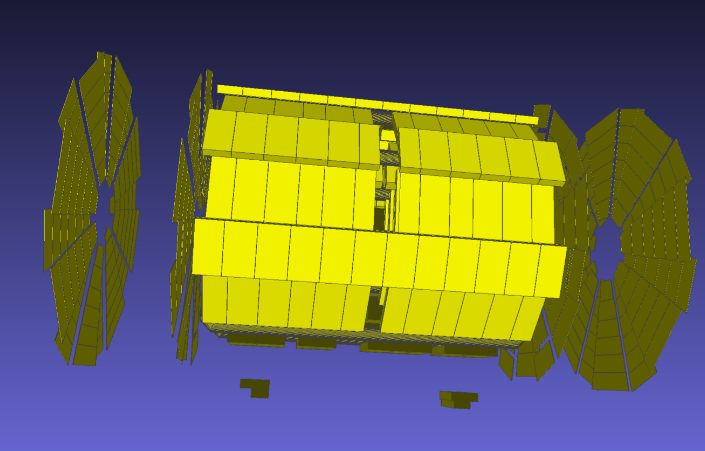
\includegraphics[width=0.8\textwidth]{figures/reco/reco_acts_muon_mockup.png}
  \caption{Mockup of the ATLAS Muon Spectrometer geometry in ACTS, used for proof-of-concept purposes.}\label{fig:reco_acts_muon_mockup}
\end{figure}

Following the initial proof-of-concept, the mockup geometry was replaced with a complete description of the muon detector and integrated into Athena. This updated geometry was built on the Gen 2 geometry model, as illustrated in Figure~\ref{fig:reco_acts_muon_gen2}, which includes all components of the muon system. In the figure, volumes are color-coded: green indicates a portal with two established links, while red (if present) would signify a portal with a missing link. The entire muon system is enclosed within a dedicated world volume, whose sole purpose is to host the frustum-based navigation model used for identifying candidate volumes. Furthermore, each volume is populated with its corresponding sensitive surfaces. A detailed view of an MDT chamber, including its straw tubes, is shown in Figure~\ref{fig:reco_acts_muon_sensitives_gen2}.

\begin{figure}[htp]
  \centering
  \subfloat[Muon Gen 2 Geometry]{
    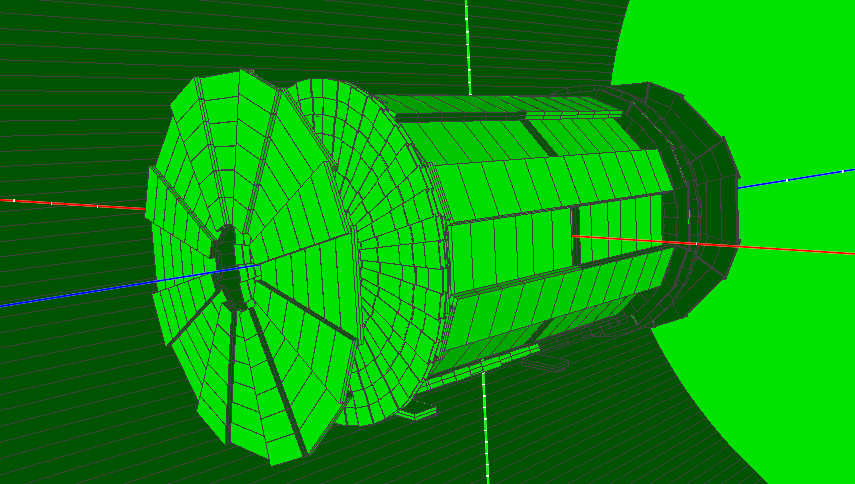
\includegraphics[width=0.48\textwidth,height=0.4\textwidth]{figures/reco/reco_acts_muon_gen2.png}\label{fig:reco_acts_muon_gen2}
  }
  \hfill
  \subfloat[MDT sensitives in Gen 2 Geometry]{
    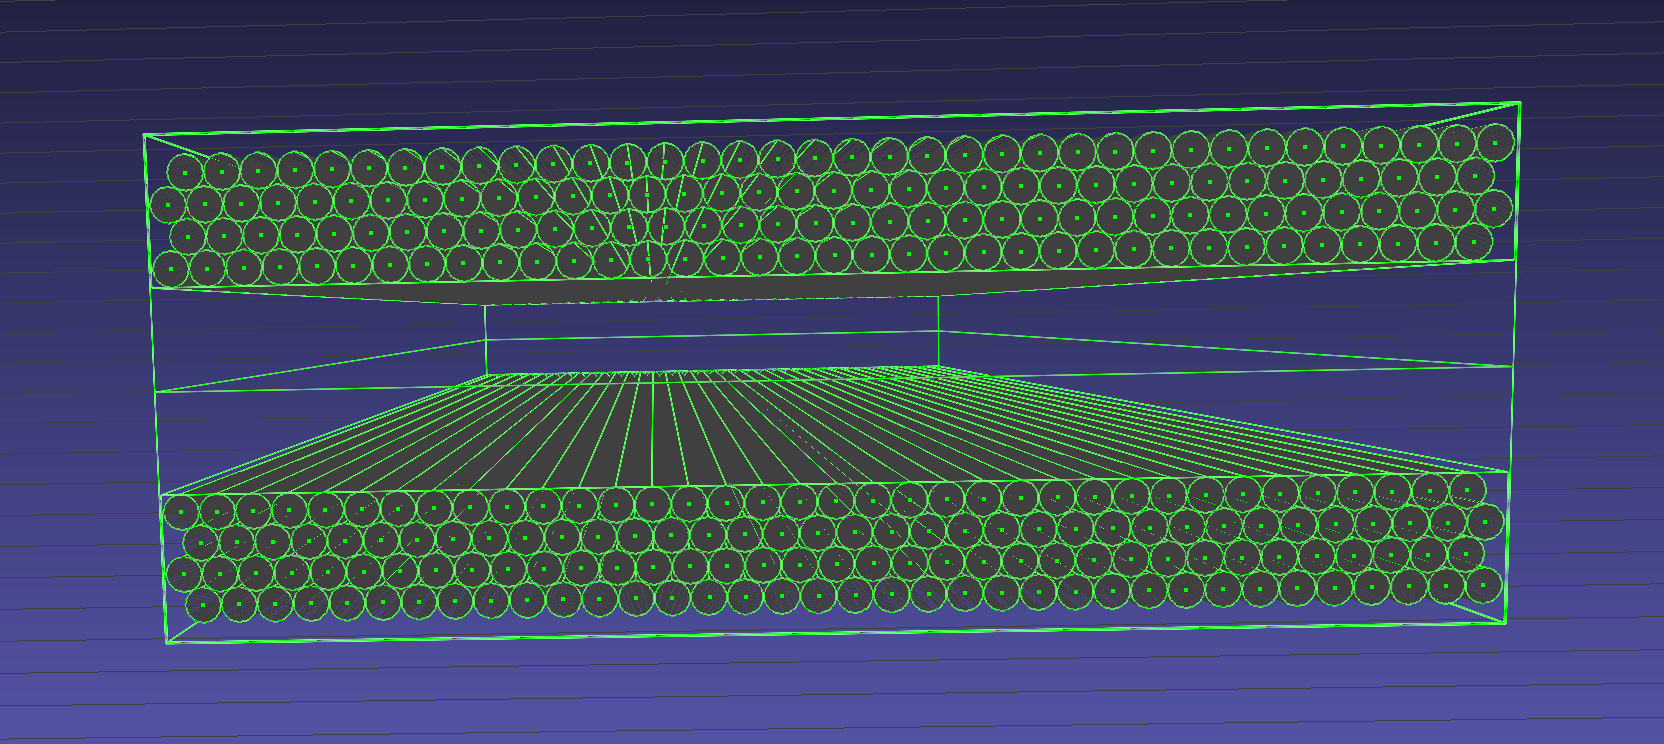
\includegraphics[width=0.48\textwidth,height=0.4\textwidth]{figures/reco/reco_acts_muon_sensitives_gen2.png}\label{fig:reco_acts_muon_sensitives_gen2}
  }
  \caption{Left: the full Muon Gen 2 geometry. Right: the interior of an MDT chamber showing sensitive elements such as straw tubes.}\label{fig:reco_acts_muon_and_sensitives_gen2}
\end{figure}

An initial implementation of passive material description was also carried out using the Gen 2 geometry. For active materials, the approach involves blending all materials within a chamber and assigning the resulting composition to a surface positioned at the center of the chamber. More complex structures, such as support elements, are currently approximated using a homogeneous volume-based material description applied to bounding boxes that encapsulating the chambers. The support components often have irregular shapes, including oddly shaped edges and holes. While this simplified approach provides a starting point for passive material modelling, it remains a rough approximation and requires significant refinement to achieve a realistic description.

To validate the Gen 2 muon geometry, debugging was performed within Athena using a `try-all' navigation strategy, which systematically checks every volume. After propagation, the resulting reconstructed hits are compared against the corresponding truth hits from the Geant4 simulation~\cite{Agostinelli:2002hh}, providing a basis for verifying verifying the truth geometry with the reconstruction geometry.
